% 79-47(79쪽) — 원 $x^{2}+y^{2}=1$ 위의 점 $\pt{P}$ 와 $x$축에 내린 수선의 발 $\pt{A}$(원문 「오른쪽 그림」). 스캔 화질이 낮아 TikZ 로 다시 그림.
% 라벨은 원문 것만: $x$·$y$·$\pt{O}$·$\pt{A}$·$\pt{P}$·$1$·$-1$·$x^{2}+y^{2}=1$, 각 $\alpha$·$\beta$, 원문처럼 삼각형 $\pt{POA}$ 를 연한 주황으로 칠한다.
% 삼각형 $\pt{POA}$ 의 넓이(답)가 그림에서 읽히지 않게 $\pt{P}$ 의 좌표·각도 눈금은 적지 않는다.
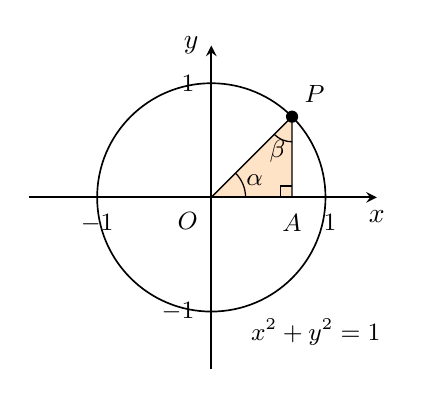
\begin{tikzpicture}[line width=0.6pt, x=1.45cm, y=1.45cm, >=stealth]
  \fill[orange!22] (0,0) -- (0.7071,0) -- (0.7071,0.7071) -- cycle;
  \draw (0,0) circle (1);
  \draw[->, line width=0.7pt] (-1.6,0) -- (1.45,0) node[below=1pt] {$x$};
  \draw[->, line width=0.7pt] (0,-1.5) -- (0,1.33) node[left=1pt] {$y$};
  \draw[line width=0.5pt] (0,0) -- (0.7071,0.7071) -- (0.7071,0);
  \draw[line width=0.45pt] (0.6071,0) -- (0.6071,0.1) -- (0.7071,0.1);
  \draw[line width=0.45pt] (0.30,0) arc (0:45:0.30);
  \draw[line width=0.45pt] (0.7071,0.7071) ++(225:0.22) arc (225:270:0.22);
  \fill (0.7071,0.7071) circle (2.2pt);
  \node[font=\small] at (0.38,0.15) {$\alpha$};
  \node[font=\small] at (0.58,0.40) {$\beta$};
  \node[font=\small, anchor=south west] at (0.73,0.74) {$\pt{P}$};
  \node[font=\small, anchor=north] at (0.7071,-0.06) {$\pt{A}$};
  \node[font=\small, anchor=north east] at (-0.03,-0.04) {$\pt{O}$};
  \node[font=\small, anchor=east] at (-0.06,1) {$1$};
  \node[font=\small, anchor=east] at (-0.06,-1) {$-1$};
  \node[font=\small, anchor=north] at (-1,-0.06) {$-1$};
  \node[font=\small, anchor=north] at (1.04,-0.06) {$1$};
  \node[font=\small, anchor=west] at (0.26,-1.18) {$x^{2}+y^{2}=1$};
\end{tikzpicture}
